% !TEX TS-program = xelatex
% !TEX encoding = UTF-8 Unicode

\providecommand{\home}{../..}
\documentclass[\home/main.tex]{subfiles}

\begin{document}

\chapter{introduction}\label{ch:introduction}


\section{Robotic laundry}
Structuur:
\begin{itemize}
    \item Droom van robot automatisatie
    \item Robotic laundry, een voorbeeld van household taak maar ook relevant voor Vlaamse industrie en breder: vervormbare objecten
    \item Traditionele robotic pipelines: hoe + waar ze falen
    \item Moderne robotic pipelines: wat ze oplossen maar waar we nog tekort schieten (single focus op rigide objecten, grote datasets of veel exp nodig en reward hacking).
    \item Insert figure~\ref{fig:intro_end2end} maar hermaak met eigen beelden!
\end{itemize}

\begin{figure}
    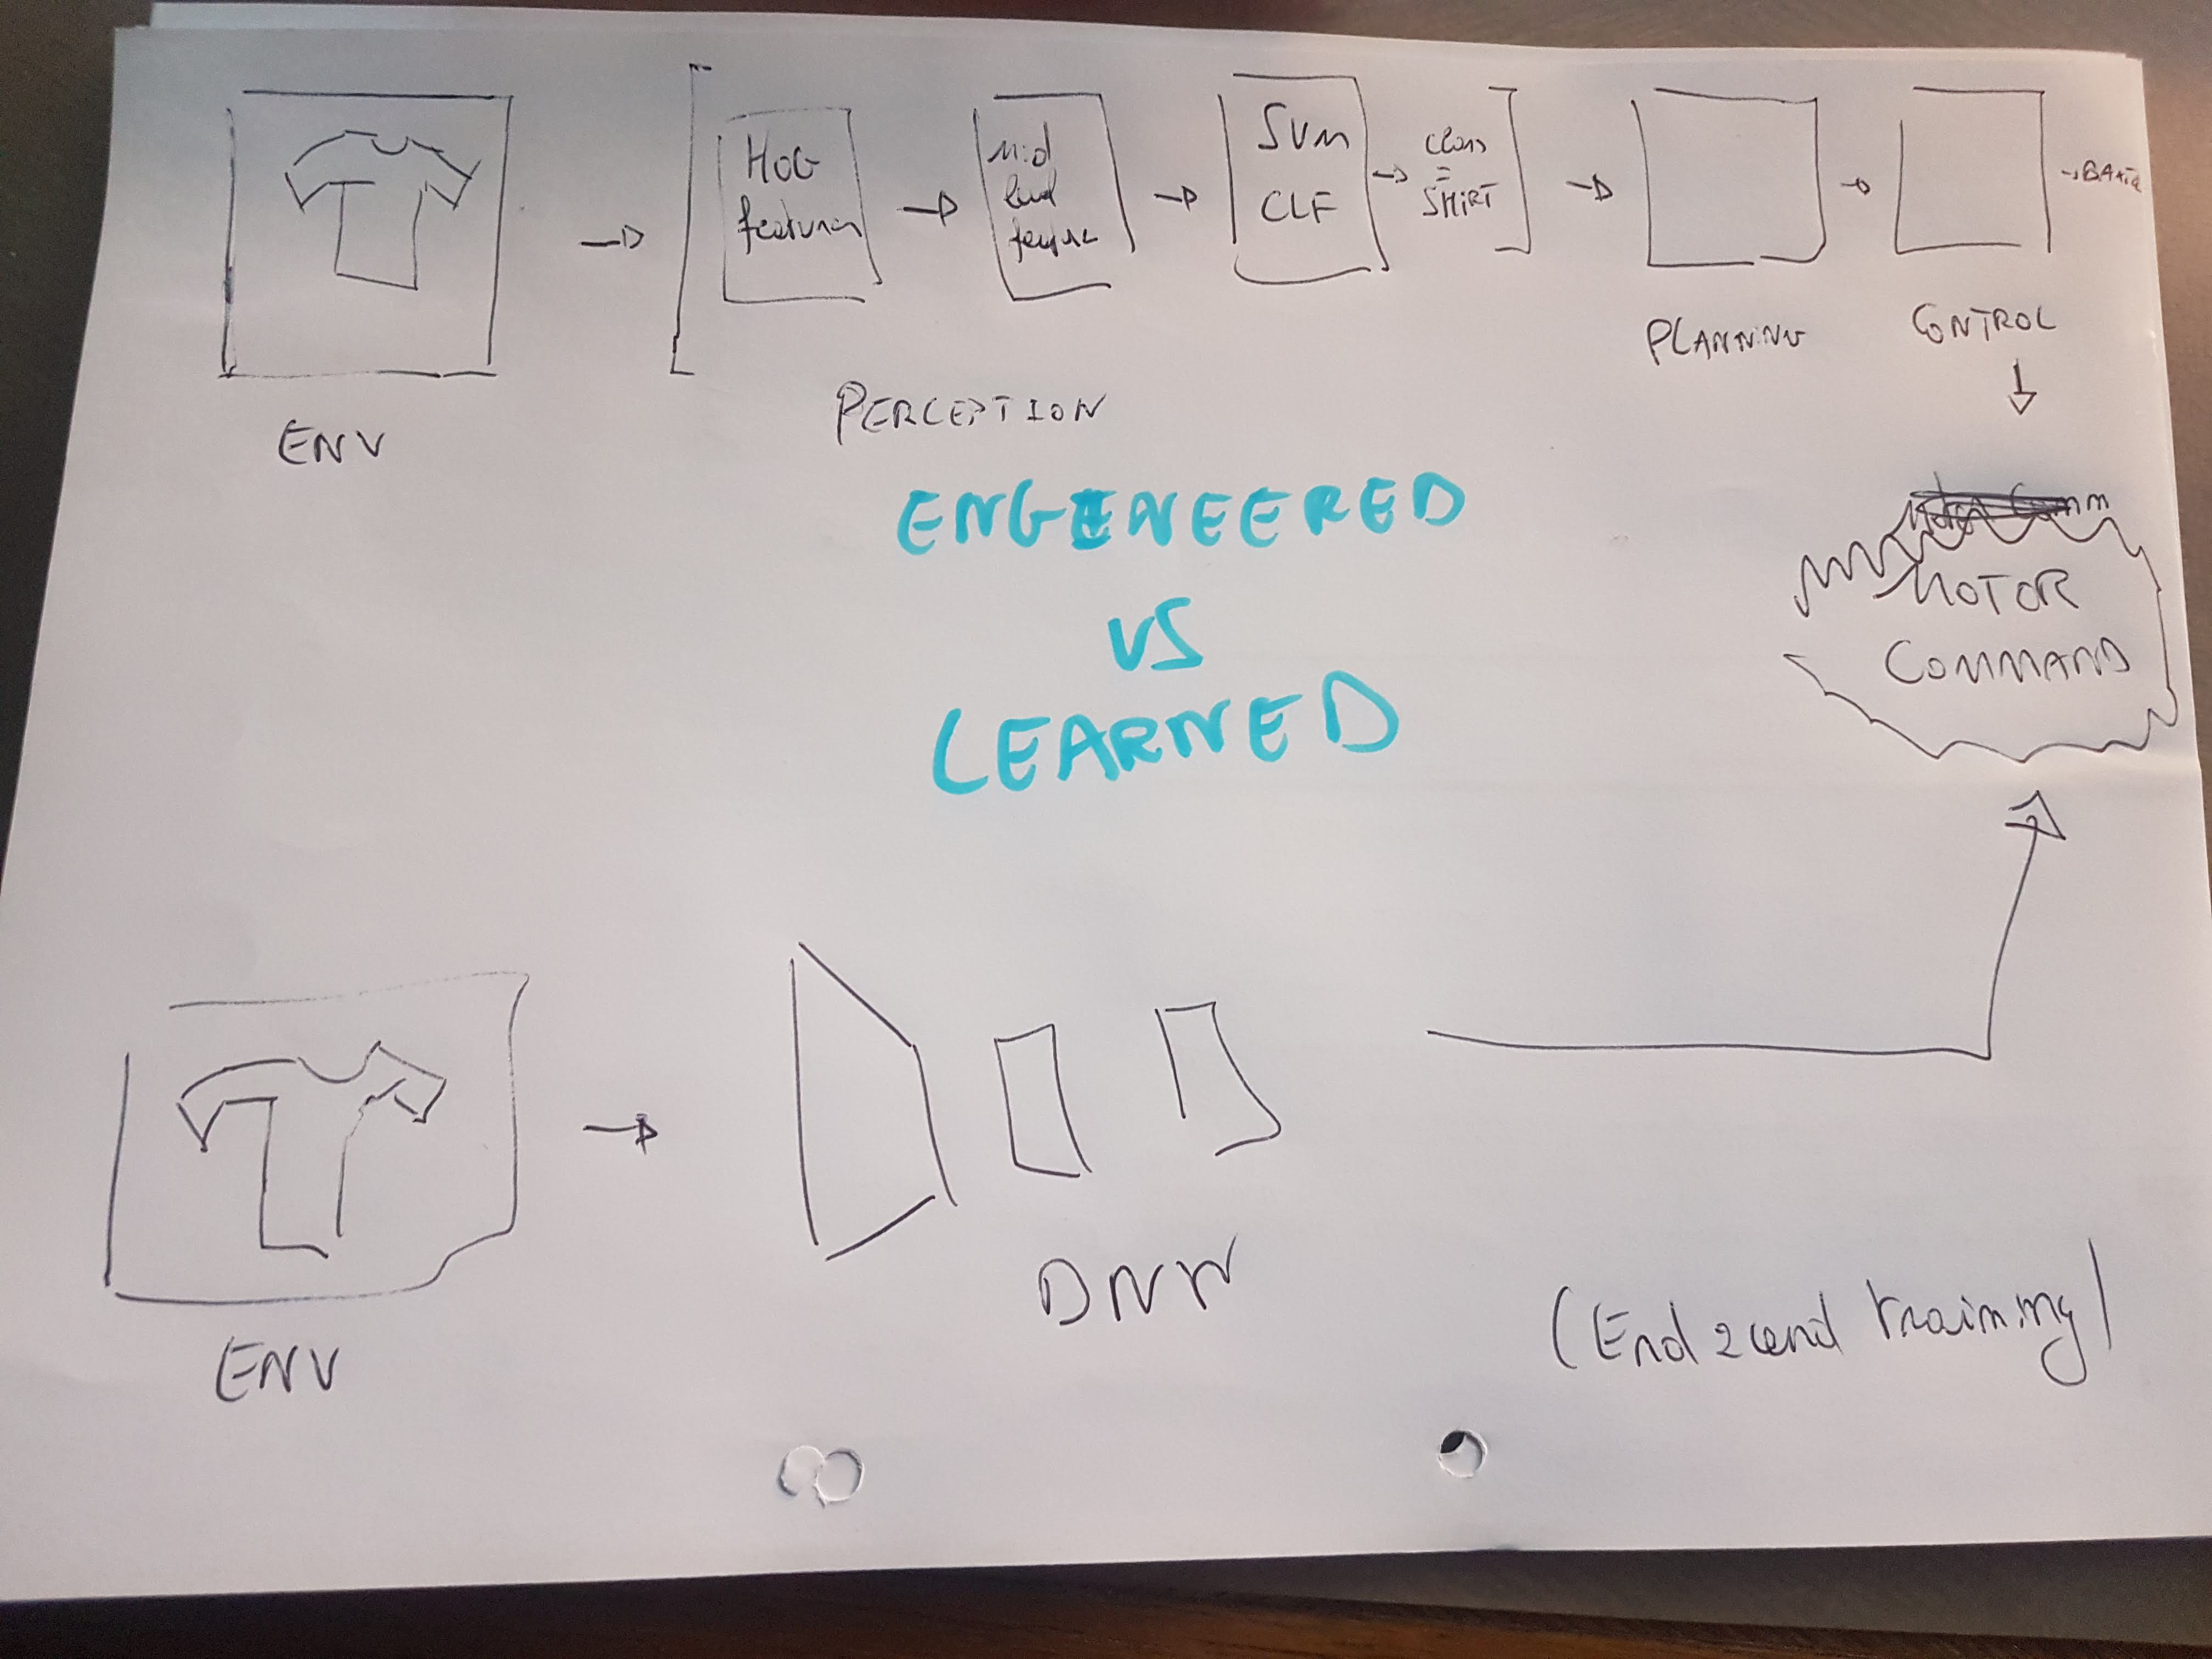
\includegraphics[width=\linewidth]{\home/chapters/01-introduction/figures/end2end-mockup}
    \caption{\textbf{Standard robotic control pipelines versus end-to-end architectures.} The diagram on the top shows how an image is processed to manually tuned features in order to do state estimation. This is then used downstream for trajectory planning and motor control. The diagram on the bottom shows an end-to-end approach to the same problem: an image is given to a deep neural network that learns its own features and executes actions directly on the actuators.}
    \label{fig:intro_end2end}
\end{figure}

\section{Accelerating robotic learning}
\subsection{Datasets}
\subsection{Simulation}
\subsection{Instrumentation}
\section{From behavioral cloning to understanding task intent}
\section{Research contributions} \label{sec:intro_contributions}
\begin{itemize}
    \item Dataset with people folding clothing
    \item Unsupervised reward function
    \item Low-cost robot setup to fold cloth invivo
    \item Instrumentation
    \item Gripper for folding
\end{itemize}

\section{Thesis structure}
This thesis is structured to first provide preliminary background and a review of the relevant literature. The remainder of the thesis deals with the methodology and results iterated in the previous Section~\ref{sec:intro_contributions}. The structure is as follows:
\begin{itemize}
    \item In Chapter~\ref{ch:lit}, we
\end{itemize}


\end{document}
